\chapter{Production Deployment and Inference Optimization}

\section*{Why This Matters}

Production deployment represents the operational phase where models deliver business value. While training is a one-time investment, inference costs are ongoing operational expenses that scale with usage. For high-volume applications serving millions of requests daily, inference costs can exceed training costs within weeks or months.

Understanding inference optimization techniques, serving architectures, and deployment trade-offs is essential for accurate cost forecasting, infrastructure planning, and vendor evaluation. A model that costs \$50,000 to train might cost \$500,000 annually to serve at scale—making deployment efficiency a primary economic concern.

This chapter examines production deployment from an engineering and economic perspective, focusing on optimization techniques, serving architectures, and the trade-offs that determine deployment costs and performance.

\section{Inference Versus Training Requirements}

\subsection{Resource Profile Differences}

Inference and training present fundamentally different resource requirements and optimization opportunities.

\textbf{Memory Requirements}: Inference eliminates gradients, optimizer states, and large activation batches required for training. BERT-base requires approximately 6 GB for training but only 500 MB for inference—a 12× reduction. This disparity enables deployment on less expensive hardware or higher throughput on given hardware.

\textbf{Computational Patterns}: Training performs forward and backward passes; inference performs only forward passes. This halves computational requirements per input. Additionally, inference typically processes smaller batches (1-32 sequences) versus training batches (32-512 sequences), changing memory access patterns and optimization opportunities.

\textbf{Latency Sensitivity}: Training tolerates variable latency—a batch taking 0.5 seconds versus 0.6 seconds rarely matters. Inference often requires strict latency guarantees—99th percentile latency under 100ms for interactive applications. This constraint shapes optimization strategies and infrastructure choices.

\subsection{Optimization Priorities}

Training optimization prioritizes throughput—maximizing tokens processed per dollar. Inference optimization balances multiple objectives:

\textbf{Latency}: Time from request to response. Critical for interactive applications (chatbots, search). Target latencies range from 50ms (search) to 500ms (content generation).

\textbf{Throughput}: Requests processed per second per server. Determines infrastructure costs for high-volume applications.

\textbf{Cost}: Infrastructure expenses per million requests. Combines hardware costs, utilization rates, and operational overhead.

These objectives often conflict. Optimizing for minimum latency (small batches, dedicated hardware) increases cost per request. Optimizing for minimum cost (large batches, shared hardware) increases latency. Production deployments navigate these trade-offs based on application requirements.


\section{Model Compression Techniques}

\subsection{Quantization}

Quantization reduces numerical precision from 32-bit or 16-bit floating-point to 8-bit integers, decreasing model size and increasing inference speed.

\textbf{Post-Training Quantization}: Converts trained model weights to lower precision without retraining. For BERT-base, 8-bit quantization reduces model size from 440 MB to 110 MB (4× reduction) with typically $<$1\% accuracy degradation. Implementation requires calibration on representative data to determine optimal quantization parameters.

\textbf{Quantization-Aware Training}: Simulates quantization during training, enabling the model to adapt to reduced precision. This approach achieves better accuracy than post-training quantization, often maintaining full precision performance while using 8-bit inference.

\textbf{Performance Benefits}: Modern CPUs and GPUs include specialized 8-bit arithmetic instructions providing 2-4× throughput compared to 32-bit operations. For BERT-base on CPU, quantization typically provides 3× speedup with 4× memory reduction.

\subsection{Knowledge Distillation}

Knowledge distillation trains a smaller "student" model to replicate a larger "teacher" model's behavior, achieving comparable performance with fewer parameters.

\textbf{Distillation Process}: The student model trains on both ground-truth labels and teacher model predictions. Teacher predictions provide richer training signal than labels alone, enabling smaller models to achieve higher accuracy than training from scratch.

\textbf{Typical Results}: DistilBERT (66M parameters) achieves 97\% of BERT-base (110M parameters) performance with 40\% fewer parameters and 60\% faster inference. For production deployment, this translates to 40\% lower infrastructure costs with minimal quality degradation.

\textbf{Implementation Considerations}: Distillation requires access to teacher model during student training, increasing training costs. However, for high-volume applications, deployment savings justify distillation investment within days or weeks.

\subsection{Pruning}

Pruning removes parameters with minimal impact on model performance, reducing model size and computational requirements.

\textbf{Unstructured Pruning}: Removes individual weights based on magnitude or importance metrics. Can achieve 50-80\% sparsity (parameter removal) with $<$1\% accuracy loss. However, unstructured sparsity provides limited speedup on standard hardware without specialized sparse computation libraries.

\textbf{Structured Pruning}: Removes entire neurons, attention heads, or layers, producing models that run efficiently on standard hardware. Typical results: 30-40\% parameter reduction with 1-2\% accuracy loss and proportional speedup.

\textbf{Practical Application}: Structured pruning is more practical for production deployment due to hardware compatibility. Removing 4 of 12 attention heads reduces computation by 33\% with minimal accuracy impact, requiring no specialized hardware or libraries.

\begin{figure}[htbp]
\centering
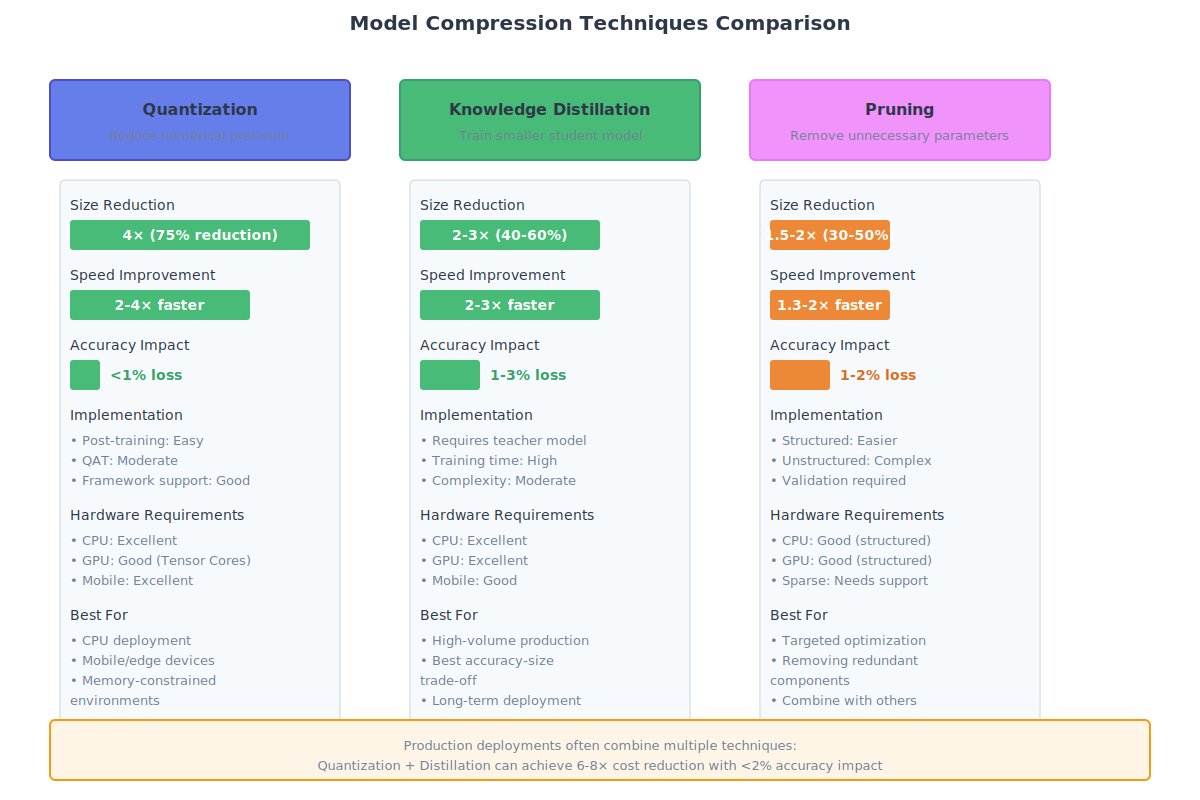
\includegraphics[width=0.95\textwidth]{chapters/diagrams/chapter05_compression_comparison_a1b2c3d4.pdf}
\caption{Model compression techniques comparison. Quantization provides best speed-memory trade-off; distillation provides best accuracy-size trade-off; pruning enables targeted optimization. Production deployments often combine multiple techniques.}
\label{fig:compression_comparison}
\end{figure}

\begin{tcolorbox}[colback=cyan!5!white,colframe=cyan!75!black,title=\textbf{MENTAL MODEL: Compression-Quality Frontier}]

\textbf{Principle:} Most models can be compressed 2-4× with less than 1\% accuracy loss. Beyond that, quality degrades rapidly.

\textbf{The Compression Ladder:}

\textbf{Level 1 (2× compression, less than 0.5\% accuracy loss):}
\begin{itemize}
    \item INT8 quantization (post-training)
    \item Effort: 1-2 days, Cost: \$0
    \item Use: Always—no reason not to
\end{itemize}

\textbf{Level 2 (3-4× compression, less than 1\% accuracy loss):}
\begin{itemize}
    \item Knowledge distillation (train smaller model)
    \item Effort: 1-2 weeks, Cost: \$2K-5K
    \item Use: When serving greater than 10M requests/month
\end{itemize}

\textbf{Level 3 (4-8× compression, 1-3\% accuracy loss):}
\begin{itemize}
    \item Aggressive pruning plus quantization
    \item Effort: 2-4 weeks, Cost: \$5K-10K
    \item Use: When cost savings (greater than \$50K/year) justify quality trade-off
\end{itemize}

\textbf{Level 4 (greater than 8× compression, greater than 3\% accuracy loss):}
\begin{itemize}
    \item Extreme compression (4-bit quantization, 90\% pruning)
    \item Effort: 1-2 months, Cost: \$10K-20K
    \item Use: Rarely—usually better to redesign architecture
\end{itemize}

\textbf{Decision Framework:}
\begin{enumerate}
    \item Start with Level 1 (INT8)—always worth it
    \item Calculate annual inference cost at current volume
    \item If greater than \$100K/year, invest in Level 2 (distillation)
    \item If greater than \$500K/year and 1-3\% quality loss acceptable, consider Level 3
    \item Never go to Level 4—redesign instead
\end{enumerate}

\textbf{Example:} Serving 50M requests/month at \$0.002/request equals \$100K/month equals \$1.2M/year. Level 2 compression (3× reduction) saves \$800K/year. Investment: \$5K. ROI: 160× in year 1.

\textbf{Red Flag:} "We need 10× compression"—this usually indicates wrong model choice. A properly-sized model with 2-4× compression beats an oversized model with 10× compression.

\end{tcolorbox}

\section{Inference Optimization Techniques}

\subsection{Operator Fusion}

Operator fusion combines multiple operations into single optimized kernels, reducing memory traffic and improving performance.

\textbf{Attention Fusion}: Standard attention implementation performs query-key multiplication, softmax, and attention-value multiplication as separate operations. Fused attention (Flash Attention, xFormers) combines these into a single kernel, reducing memory traffic by 3-4× and providing 2-4× speedup.

\textbf{Layer Fusion}: Combines layer normalization, activation functions, and residual connections into fused operations. For transformer layers, fusion typically provides 10-20\% speedup with no accuracy impact.

\textbf{Framework Support}: Modern frameworks (PyTorch 2.0, TensorFlow, ONNX Runtime) provide automatic fusion through compilation. Manual fusion using custom CUDA kernels can provide additional 20-30\% speedup but requires significant engineering investment.

\subsection{Batching Strategies}

Batching—processing multiple requests together—improves GPU utilization and throughput but increases latency.

\textbf{Static Batching}: Accumulates requests until batch size threshold is reached or timeout expires, then processes batch. Simple to implement but introduces latency variance. For batch size 32 with 100ms timeout, average latency increases by 50ms compared to single-request processing.

\textbf{Dynamic Batching}: Continuously processes available requests in variable-size batches, balancing latency and throughput. More complex to implement but provides better latency-throughput trade-off. Typical configuration: maximum batch size 32, maximum wait time 10ms.

\textbf{Continuous Batching}: Processes requests as they arrive without waiting for batch completion, enabling lower latency with high throughput. Requires careful memory management and scheduling but provides optimal latency-throughput balance for variable-length inputs.

\subsection{KV Cache Optimization}

For autoregressive generation (text generation, translation), key-value (KV) cache optimization significantly improves performance and represents one of the highest-ROI production optimizations.

\textbf{KV Cache Mechanism}: During generation, attention keys and values from previous tokens are cached and reused, avoiding recomputation. For a 512-token generation, KV caching reduces computation by approximately 500× compared to recomputing from scratch each step.

\textbf{Memory Requirements}: KV cache memory scales with sequence length and batch size. For BERT-base generating 512 tokens with batch size 8, KV cache requires approximately 2 GB. This memory overhead limits batch sizes for long-sequence generation.

\textbf{Multi-Query Attention (MQA) and Grouped-Query Attention (GQA)}: By 2026, these techniques have become standard for production inference, not optional optimizations. They reduce KV cache by 4-8× with <1\% quality degradation:

For LLaMA 2 scale models:
\begin{itemize}
    \item Standard attention: 1.6 GB KV cache per batch of 32
    \item GQA (8 groups): 200 MB KV cache
    \item Impact: 40-80\% inference throughput improvement on memory-bound workloads
\end{itemize}

These should be default choices for production inference, not optimization afterthoughts. The memory savings enable larger batch sizes, directly improving throughput and reducing per-request costs.

\textbf{PagedAttention}: Recent optimization technique that manages KV cache memory more efficiently through paging, similar to virtual memory in operating systems. This approach increases achievable batch size by 2-3× for long-sequence generation, proportionally improving throughput. Combined with GQA, PagedAttention enables 6-10× throughput improvements for long-context generation.


\section{Serving Architectures}

\subsection{Model Serving Patterns}

Production deployments employ various serving patterns based on latency requirements, throughput needs, and cost constraints.

\textbf{Dedicated Model Servers}: Each model runs on dedicated hardware with isolated resources. This pattern provides predictable latency and simplifies capacity planning but increases costs for multiple models. Appropriate for high-volume, latency-sensitive applications.

\textbf{Multi-Model Serving}: Multiple models share hardware resources, improving utilization and reducing costs. Requires careful resource allocation and scheduling to prevent interference. Appropriate for lower-volume models or when latency requirements are relaxed.

\textbf{Serverless Deployment}: Models deployed as serverless functions that scale automatically with demand. Provides excellent cost efficiency for variable or unpredictable load but introduces cold-start latency (1-5 seconds typically). Appropriate for batch processing or asynchronous workflows.

\begin{figure}[htbp]
\centering
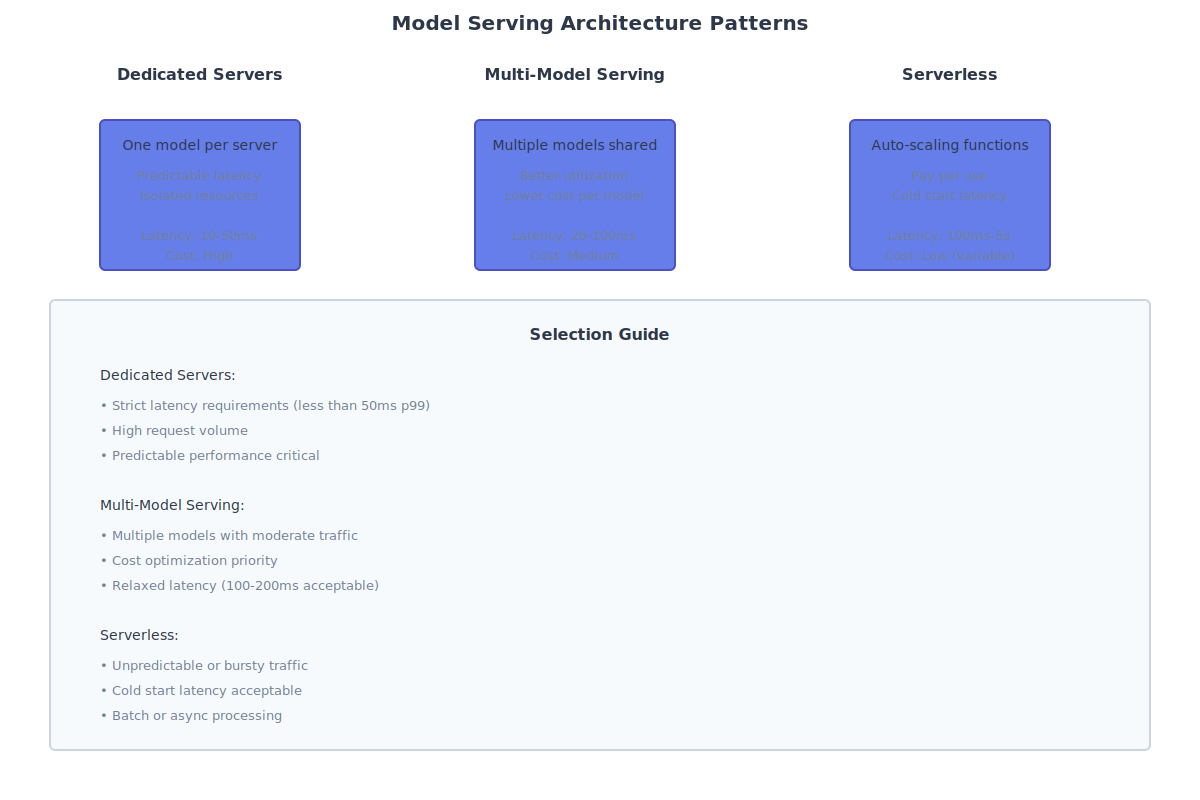
\includegraphics[width=0.9\textwidth]{chapters/diagrams/chapter05_serving_architecture_e5f6g7h8.pdf}
\caption{Model serving architecture patterns. Dedicated servers provide lowest latency; multi-model serving provides best resource utilization; serverless provides best cost efficiency for variable load. Choice depends on latency requirements and usage patterns.}
\label{fig:serving_architecture}
\end{figure}

\subsection{Load Balancing and Scaling}

Effective load balancing and scaling strategies ensure consistent performance under variable load.

\textbf{Horizontal Scaling}: Adds more model server instances to handle increased load. Provides linear scaling for stateless inference but requires load balancer and health monitoring. Typical scaling policy: add instance when CPU utilization exceeds 70\%, remove when below 30\%.

\textbf{Vertical Scaling}: Uses larger instances with more GPUs or memory. Simpler than horizontal scaling but limited by maximum instance size. Appropriate when single-instance performance is insufficient.

\textbf{Auto-Scaling}: Automatically adjusts instance count based on metrics (request rate, latency, utilization). Essential for variable load patterns. Typical configuration: scale up aggressively (30-60 seconds), scale down conservatively (5-10 minutes) to prevent oscillation.

\subsection{Caching Strategies}

Caching reduces inference costs by storing and reusing results for repeated requests.

\textbf{Result Caching}: Caches complete inference results keyed by input. Highly effective for repeated queries (FAQ systems, common searches). Cache hit rates of 30-50\% are common, reducing infrastructure costs proportionally.

\textbf{Embedding Caching}: Caches intermediate representations (embeddings) for frequently-accessed content. Useful for retrieval systems where document embeddings are computed once and reused for multiple queries.

\textbf{Cache Invalidation}: Determines when cached results become stale. Simple time-based expiration (TTL) works for most applications. More sophisticated approaches track model version and invalidate on updates.


\section{Deployment Platforms and Trade-offs}

\subsection{Cloud Deployment}

Cloud platforms (AWS, GCP, Azure) provide managed infrastructure with flexible scaling but introduce ongoing costs.

\textbf{Managed Services}: Platforms like AWS SageMaker, GCP Vertex AI, Azure ML provide fully-managed model serving with automatic scaling, monitoring, and updates. Simplifies operations but costs 20-40\% more than self-managed infrastructure.

\textbf{Container-Based Deployment}: Deploy models in containers (Docker, Kubernetes) on cloud VMs. Provides flexibility and cost efficiency but requires more operational expertise. Typical cost: \$2-4/hour for GPU instances (A100), \$0.10-0.30/hour for CPU instances.

\textbf{Spot Instances}: Use preemptible instances at 60-80\% discount for fault-tolerant workloads. Requires graceful handling of instance termination. Appropriate for batch processing or when redundancy enables tolerance of individual instance failures.

\subsection{On-Premises Deployment}

On-premises deployment provides control and potentially lower long-term costs but requires capital investment and operational expertise.

\textbf{Capital Costs}: GPU servers cost \$50,000-150,000 depending on configuration (A100 servers typically \$100,000-120,000). Amortized over 3-year lifetime: approximately \$3,000-4,000/month per server.

\textbf{Operational Costs}: Power, cooling, networking, and maintenance add 30-50\% to hardware costs. A 10-server GPU cluster costs approximately \$40,000-60,000/month including all operational expenses.

\textbf{Break-Even Analysis}: On-premises deployment becomes cost-effective at sufficient scale. For continuous GPU utilization, break-even typically occurs at 6-12 months compared to cloud deployment. For variable utilization, cloud deployment often remains more cost-effective.

\subsection{Edge Deployment}

Edge deployment runs models on user devices or edge servers, reducing latency and cloud costs but constraining model size.

\textbf{Mobile Deployment}: Models run on smartphones or tablets. Requires aggressive compression (quantization, distillation) to fit memory constraints (typically $<$100 MB) and power constraints. Appropriate for privacy-sensitive applications or offline functionality.

\textbf{Edge Servers}: Deploy models on edge servers closer to users, reducing latency from 100-200ms (cloud) to 10-30ms (edge). Requires distributed deployment and management but provides better user experience for latency-sensitive applications.

\textbf{Hybrid Approaches}: Combine edge and cloud deployment, running small models on-device for common cases and falling back to cloud for complex cases. Balances latency, cost, and capability.

\begin{figure}[htbp]
\centering
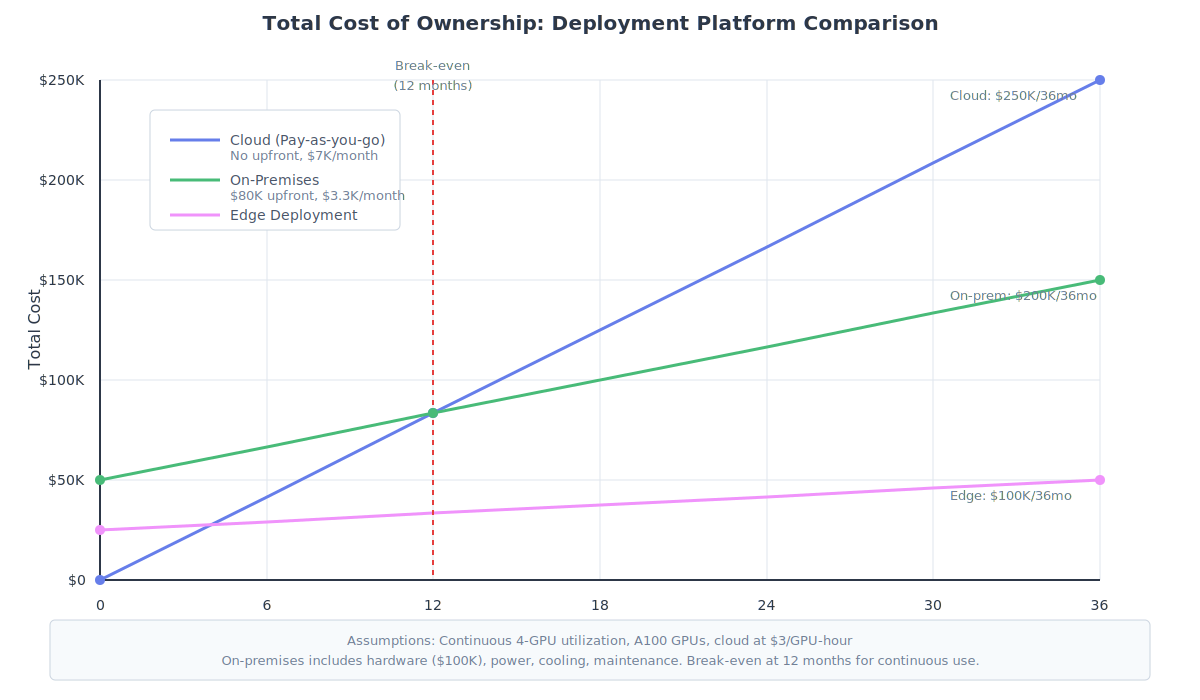
\includegraphics[width=0.9\textwidth]{chapters/diagrams/chapter05_deployment_costs_i9j0k1l2.pdf}
\caption{Deployment cost comparison across platforms. Cloud provides flexibility; on-premises provides lower long-term costs at scale; edge provides lowest latency and ongoing costs. Choice depends on scale, utilization patterns, and latency requirements.}
\label{fig:deployment_costs}
\end{figure}


\section{Cost Analysis and Optimization}

\subsection{Inference Cost Breakdown}

Understanding cost components enables targeted optimization:

\textbf{Compute Costs} (60-70\%): GPU or CPU rental/amortization. For cloud deployment with A100 GPUs at \$3/hour, processing 1 million BERT-base requests (50ms each) costs approximately \$42 in compute time.

\textbf{Memory and Storage} (10-15\%): Model storage, KV cache memory, and intermediate results. Larger models or longer sequences increase memory costs proportionally.

\textbf{Network Costs} (10-15\%): Data transfer between services and to users. For cloud deployment, egress costs can be significant—typically \$0.08-0.12/GB.

\textbf{Operational Overhead} (10-15\%): Monitoring, logging, load balancing, and management infrastructure. Often underestimated but essential for production reliability.

\subsection{Cost Optimization Strategies}

Several strategies reduce inference costs without compromising quality:

\textbf{Model Compression}: Quantization and distillation reduce costs by 2-4× with minimal accuracy impact. For a system serving 100 million requests monthly at \$0.001/request, compression reduces costs from \$100,000 to \$25,000-50,000 monthly.

\begin{tcolorbox}[colback=blue!5!white,colframe=blue!75!black,title=\textbf{IN PRACTICE: ROI of Model Compression}]

\textbf{Scenario}: E-commerce company serving 100M product recommendations/month

\textbf{Before Compression} (BERT-base, FP32):
\begin{itemize}
    \item Model size: 440 MB
    \item Latency: 50ms per request
    \item Infrastructure: 20× A100 GPUs
    \item Monthly cost: \$100,000
\end{itemize}

\textbf{After Compression} (8-bit quantization + distillation):
\begin{itemize}
    \item Model size: 110 MB (4× reduction)
    \item Latency: 18ms per request (2.8× faster)
    \item Infrastructure: 8× A100 GPUs (60\% reduction)
    \item Monthly cost: \$40,000
    \item Accuracy impact: -0.3\% (negligible)
\end{itemize}

\textbf{Investment vs. Return}:
\begin{itemize}
    \item Engineering cost: 2 weeks × \$10k/week = \$20,000
    \item Monthly savings: \$60,000
    \item Payback period: 10 days
    \item Annual savings: \$720,000
\end{itemize}

\textbf{Lesson}: For high-volume applications, compression engineering pays for itself within days.

\end{tcolorbox}

\textbf{Batching Optimization}: Increasing batch size from 1 to 16 typically improves throughput by 8-12×, reducing per-request costs proportionally. Requires balancing against latency requirements.

\textbf{Hardware Selection}: CPU inference costs 5-10× less than GPU inference for small models or low throughput. For BERT-base with $<$10 requests/second, CPU deployment is more cost-effective. Above 50 requests/second, GPU deployment becomes more economical.

\textbf{Caching}: Result caching with 30\% hit rate reduces infrastructure costs by 30\%. Implementation cost is minimal—typically a Redis or Memcached cluster costing $<$5\% of inference infrastructure.

\subsection{Cost Forecasting}

Accurate cost forecasting requires understanding scaling relationships:

\begin{center}
\fbox{\parbox{0.85\textwidth}{
\centering
Monthly Cost = (Requests/Month) $\times$ (Latency/Request) $\times$ (GPU Cost/Hour) / (3600 $\times$ Batch Size $\times$ Utilization)
}}
\end{center}

For 100 million monthly requests, 50ms latency, \$3/hour GPU cost, batch size 16, 60\% utilization:

Monthly Cost = 100M $\times$ 0.05 $\times$ 3 / (3600 $\times$ 16 $\times$ 0.6) $\approx$ \$43,000

This formula enables rapid cost estimation for different scenarios and optimization strategies.


\section{Retrieval-Augmented Generation (RAG)}

\subsection{RAG Architecture}

RAG combines retrieval systems with generative models, enabling models to access external knowledge without retraining. This fundamentally changes the cost structure of LLM applications.

\textbf{Architecture Components}: RAG systems include a retrieval component (vector database, search engine) and a generation component (language model). User queries trigger retrieval of relevant documents, which are provided as context to the language model for generation.

\textbf{Benefits}: RAG enables models to access current information, cite sources, and reduce hallucination. For enterprise applications, RAG provides access to proprietary knowledge without expensive model retraining. RAG also enables dynamic knowledge updates without retraining—a critical advantage for rapidly-changing domains.

\textbf{Cost Implications and Economics}: RAG adds retrieval costs (vector database queries, embedding computation) to generation costs. However, RAG often enables use of smaller language models since external knowledge reduces model size requirements.

For 1M queries/month:
\begin{itemize}
    \item Base LLM cost (7B model): \$3,000-5,000
    \item Retrieval cost (embedding model + vector DB): \$500-2,000
    \item Total monthly: \$3,500-7,000
    \item vs. Fine-tuned equivalent (70B model): \$30,000-50,000
\end{itemize}

RAG enables 4-7× cost reduction compared to larger models for comparable performance. Net cost impact varies by application but is often neutral or positive when accounting for the ability to use smaller base models.

\subsection{Implementation Considerations}

Effective RAG implementation requires attention to several technical details:

\textbf{Retrieval Quality}: Retrieval accuracy directly impacts generation quality. Poor retrieval provides irrelevant context, degrading output quality. Typical approach: retrieve top-k documents (k=3-10), rerank using cross-encoder, provide top-3 to generator.

\textbf{Context Length Management}: Retrieved documents must fit within model context window. For models with 2048-token context, retrieved content typically limited to 1000-1500 tokens, leaving room for query and generation.

\textbf{Latency Considerations}: RAG adds retrieval latency (typically 20-50ms) to generation latency. For latency-sensitive applications, this overhead requires optimization through caching, parallel retrieval, or approximate search.

\begin{figure}[htbp]
\centering
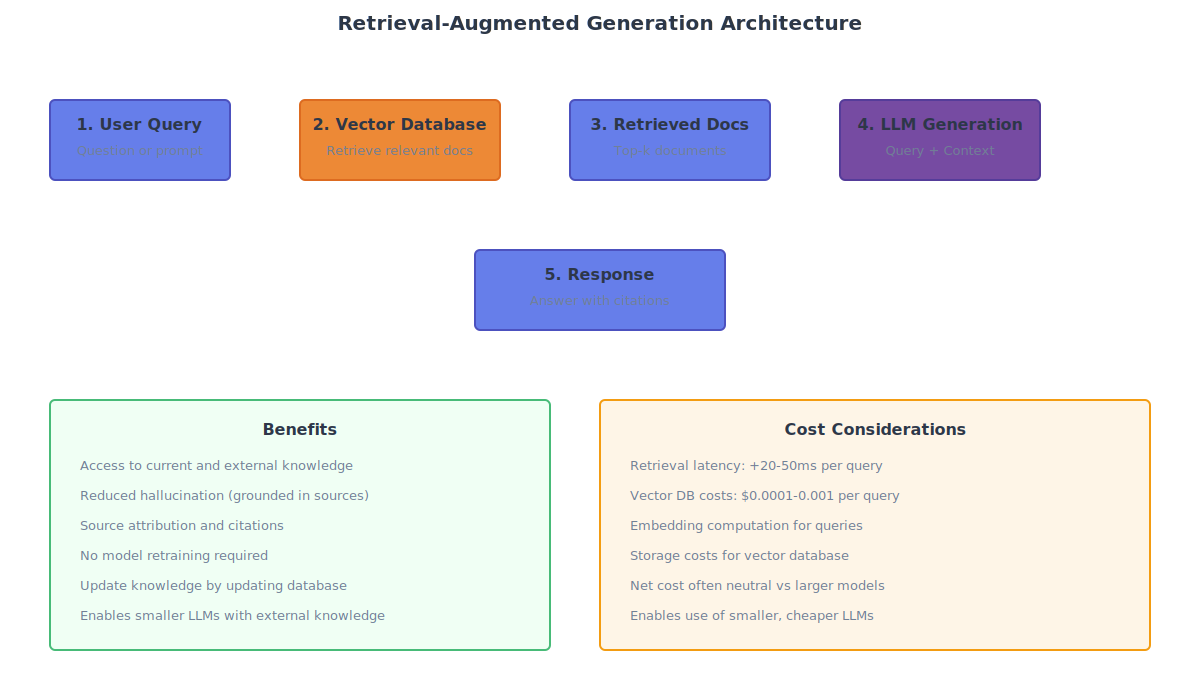
\includegraphics[width=0.95\textwidth]{chapters/diagrams/chapter05_rag_architecture_m3n4o5p6.pdf}
\caption{Retrieval-Augmented Generation architecture. User query triggers document retrieval from vector database, retrieved documents provide context for language model generation. This architecture enables access to external knowledge without model retraining.}
\label{fig:rag_architecture}
\end{figure}


\section{Monitoring and Observability}

\subsection{Performance Metrics}

Production deployments require comprehensive monitoring to ensure reliability and performance:

\textbf{Latency Metrics}: Track p50, p95, p99 latency. p99 latency (99th percentile) is critical for user experience—1\% of users experiencing 10× higher latency is unacceptable for most applications.

\textbf{Throughput Metrics}: Requests per second, tokens per second. Monitor trends to detect capacity issues before they impact users.

\textbf{Error Rates}: Track error types (timeouts, out-of-memory, invalid inputs) and rates. Sudden error rate increases indicate infrastructure or model issues requiring investigation.

\textbf{Resource Utilization}: GPU/CPU utilization, memory usage, network bandwidth. Low utilization indicates over-provisioning; high utilization indicates capacity constraints.

\subsection{Quality Monitoring}

Beyond performance metrics, monitor output quality to detect model degradation:

\textbf{Automated Quality Checks}: Implement automated checks for output validity, coherence, and safety. Flag outputs failing checks for human review.

\textbf{User Feedback}: Collect explicit feedback (thumbs up/down) and implicit feedback (engagement metrics). Declining feedback scores indicate quality issues.

\textbf{A/B Testing}: Compare model versions or configurations through controlled experiments. Essential for validating optimization impact on quality and user experience.


\section{Evaluation Framework}

\subsection{Deployment Proposal Assessment}

When evaluating deployment proposals, consider:

\textbf{Performance Requirements}:
\begin{itemize}
    \item What are the latency requirements (p50, p95, p99)?
    \item What throughput is required (requests/second, tokens/second)?
    \item What are the availability requirements (uptime percentage)?
    \item How will performance be monitored and validated?
\end{itemize}

\textbf{Optimization Strategy}:
\begin{itemize}
    \item What compression techniques are planned (quantization, distillation, pruning)?
    \item What is the expected accuracy-performance trade-off?
    \item What batching strategy will be used?
    \item Have optimization techniques been validated on representative workloads?
\end{itemize}

\textbf{Infrastructure and Costs}:
\begin{itemize}
    \item What deployment platform is proposed (cloud, on-premises, edge)?
    \item What is the estimated cost per million requests?
    \item How will the system scale with increasing load?
    \item What is the plan for cost optimization over time?
\end{itemize}

\textbf{Operational Considerations}:
\begin{itemize}
    \item What monitoring and alerting will be implemented?
    \item What is the deployment and rollback strategy?
    \item How will model updates be managed?
    \item What is the disaster recovery plan?
\end{itemize}

\subsection{Common Assessment Pitfalls}

\textbf{Underestimating Operational Complexity}: Production deployment requires monitoring, logging, alerting, and incident response. Operational costs often equal or exceed infrastructure costs.

\textbf{Ignoring Tail Latency}: Average latency is insufficient—p99 latency determines user experience. A system with 50ms average but 500ms p99 latency provides poor experience for 1\% of users.

\textbf{Inadequate Load Testing}: Proposals should include load testing results demonstrating performance under realistic conditions. Synthetic benchmarks often overestimate production performance.

\textbf{Overlooking Cost Scaling}: Linear cost scaling assumptions are often incorrect. Costs may scale super-linearly due to coordination overhead, or sub-linearly due to batching efficiency. Validate scaling assumptions through testing.


\section{Key Insights}

\textbf{Inference Dominates Long-Term Costs}: For high-volume applications, inference costs exceed training costs within weeks or months. Inference optimization provides ongoing cost savings.

\textbf{Compression Effectiveness}: Model compression (quantization, distillation) typically provides 2-4× cost reduction with $<$1\% accuracy impact. This optimization should be standard for production deployment.

\textbf{Batching Trade-offs}: Larger batches improve throughput but increase latency. Optimal batch size balances these objectives based on application requirements.

\textbf{Platform Selection}: Cloud provides flexibility; on-premises provides lower long-term costs at scale; edge provides lowest latency. Choice depends on scale, utilization patterns, and requirements.

\textbf{Monitoring Criticality}: Comprehensive monitoring is essential for production reliability. Performance and quality degradation must be detected and addressed quickly.

\textbf{RAG Viability}: Retrieval-Augmented Generation enables access to external knowledge without retraining, often at neutral or positive cost impact compared to larger models.

The next chapter examines advanced techniques—prompt engineering, fine-tuning strategies, and emerging architectural innovations that extend transformer capabilities.
